
At a high level, VITAL adds bugs to programs in the following manner.

\begin {enumerate}
\item Identify source code locations where input bytes that do not determine control flow and are still close to their original form are available. 
We call these quantities DUAs, for dead, uncomplicated and available. 
\item Find potential attack points that are temporally after a DUA in the program trace.
Attack points are source code locations where a DUA might be used, if only it were available there as well, to make a program vulnerable. 
\item Add code to the program to make the DUA value available at the attack point and use it to create the vulnerability. 
\end{enumerate}

These three steps are depicted in Figure~\ref{lava-picture} and will be discussed in the following three sections,
which refer to the worked example in Figure~\ref{worked-example}.


\begin{figure} 
\begin{tabular}{ll}
1 & \verb+ void foo(int a, int b, int c) {+ \\
2 & \verb-   int d=a+b+c;- \\
3 & \verb+   if (a == 0xdeadbeef) return;+ \\ 
4 & \verb+   memcpy(d,s,n);+ \\
5 & \verb_   // BUG_ \\
6 & \verb_   // memcpy(d+(b==0x666666)*b,s,n);_ \\
7 & \verb+ }+ \\
\end{tabular}
\caption{
VITAL worked example.  
a, b, and c are direct copies of input bytes at the start of function foo.
a is bytes 0..3, b is 4..7, and c is 8..11.
The value in b at the call to memcpy has tcn=0 and liveness=0,
so it can be used to trigger and control a vulnerability there.
}
\label{worked-example}
\end{figure}



\subsection {The DUA}

In a little more detail, the first step, in which DUAs are identified, is accomplished as follows.  

The program is executed under a dynamic taint analysis for a specific input.
That taint analysis has a few important features.
\begin{itemize}
\item Each individual byte in the input is given its own label.
Thus, if an internal program quantity is tainted and a direct copy of input bytes, then we can map that quantity back to a specific part of the input.  
\item The taint analysis operates, effectively, upon an LLVM version of the machine code for a program, including its libraries.
This means taint is propagated accurately and completely, even through esoteric x86 machine instructions like MMX and XMM.
\item The taint analysis keeps track of a \emph{set} of labels per input byte, meaning that it can represent computation that mixes input bytes.
\end{itemize}
We use the PANDA system to perform this taint analysis, with two crucial conceptual extensions in the form of taint-based measures.

The \emph{taint compute number} is a measure of how complicated a function of input bytes a tainted internal program quantity is.
TCN is illustrated in Figure~\ref{fig:taint-compute-number}; it simply tracks the depth of the tree of computation required to obtain 
a quantity from input bytes.
The smaller TCN is for a program quantity, the closer it is, computationally, to the input.
If TCN is 0, the quantity is a direct copy of input bytes.
The intuition behind this measure is that we need DUAs that are computationally close to the input in order to be able to use them with predictable results.
Note that TCN is not an ideal measure.
There are obviously situations in which the tree of computation is deep but the resulting DUA value is both completely predictable and has as much entropy as the original value.
However, TCN has the advantage that it is easy to compute.
Whenever the taint system needs to union label sets to represent computation, the TCN associated with the resulting set is one more than the max of those of the 
input sets.
TCN is an integer attached to the taint label set associated with each byte in a program.


\begin{figure}
\centering
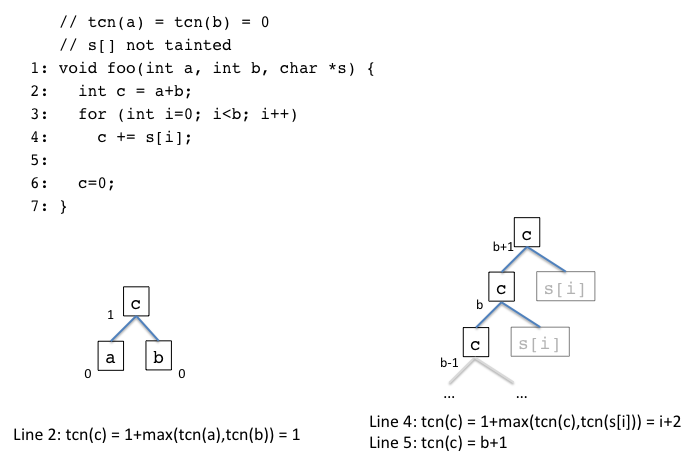
\includegraphics[width=3in]{tcn-example.png}
\caption{Taint Compute Number (TCN)}
\label{fig:taint-compute-number}
\end{figure}

%\includegraphics[natwidth=162bp,natheight=227bp]{Aston.png}


The other taint-based measure VITAL introduces is \emph{liveness}, which is associated with taint labels, i.e. the input bytes themselves.
This is a straightforward accounting of how many branches a byte in the input has been used to decide.
Thus, if a particular input byte label was never found in a taint label set associated with any byte used in a branch, it will have liveness of 0.
A DUA entirely consisting of bytes with 0 or very low liveness can be considered \emph{dead} in the sense that it has very little influence upon control flow for this program trace.
If one were to fuzz dead bytes, the program should be indifferent and execute the same trace.  

The combination of uncomplicated (low TCN) and dead (low liveness) is a powerful one for vulnerability injection.
The DUAs it identifies are internal program quantities that are often a direct copy of input bytes, and which can be set to any chosen value without sending the program along a different path.  
These make very good triggers for vulnerabilities.

In the worked example, consider the variables \verb+x+ and \verb+y+ in lines 3 and 4, respectively.
These have TCNs of 0 and 1, respectively, and liveness 0. 
These are tainted values that will make idea DUAs.

\subsection {The attack point}

Attack point identification is a function of the type of vulnerability to be injected.
If the goal is to inject a memory read overflow, then reads via pointer dereference, array index, and bulk memory copy, e.g., are reasonable attack points.  
If the goal is to inject divide-by-zero, then arithmetic operations involving division will be attacked. 
Alternately, the goal might be to control one or more arguments to a library function.
The only requirement is that the attack point be parameterized in order that it be attackable when the DUA is made available there. 

For instance, in Figure~\ref{worked-example}, on line 12, the call to \verb+memcpy+ can be attacked by introducing a data-flow relation between either \verb+x+ or \verb+y+ 
and any of the arguments to \verb+memcpy+.

\subsection {Data-flow bug injection}

The third and final step to VITAL bug injection is introducing a dataflow relationship between DUA and attack point.  
If the DUA is in scope at the attack point then it can simply be used at the attack point to introduce the vulnerability.
If it is not in scope, new code is added to copy the DUA off into a safe place (perhaps in a data structure or a global), and also retrieve it and  make use of it value at the attack point. 
However, in order to ensure that the bug only manifest itself very occasionally, we must introduce a guard requiring that the DUA match a specific value if it is to be used to manifest the vulnerability.

In the worked example in Figure~\ref{worked-example}, the DUA \verb+x+ is still in scope at the \verb+memcpy+ attack point and
 the only source code modification necessary is to make use of it to introduce the vulnerability if it matches a particular value.  









